\documentclass[brazil]{beamer}
\usepackage[brazil]{babel}
\usepackage[utf8]{inputenc}
\usepackage{graphicx}
\usetheme{Madrid}
\title[Séries Numéricas]{Séries Numéricas}
\subtitle{Convergência e Divergência}
\author[Ruas, I. P. de A.]{Isak Paulo de Andrade Ruas}
\institute[IFNMG]{
	Instituto Federal do Norte de Minas Gerais \\
	Campus Januária \\
	Curso de Licenciatura em Matemática
}
\date{5 de Dezembro de 2023}
\logo{
\includegraphics[height=1cm]{../images/logo_ifnmg.jpg}}
\usepackage{ragged2e}
\newcommand{\N}{\mathbb{N}}
\usepackage{enumitem}
\newtheorem{observation}{Observação}\theoremstyle{definition}

\begin{document}
	
	\begin{frame}[plain]
		\maketitle
	\end{frame}
	
	\begin{frame}{Agenda}
		\tableofcontents
	\end{frame}
	
	\section{Introdução às Séries Numéricas}
	\begin{frame}
		\tableofcontents[currentsection]
	\end{frame}
	
	\begin{frame}{O que são Séries Numéricas?}
		\justifying
		Uma série numérica é a soma dos termos de uma sequência infinita de números.
		Existem diferentes tipos de séries numéricas, as quais são classificadas de
		acordo com as propriedades dos termos na sequência e da maneira como eles são
		somados.
	\end{frame}
	\begin{frame}{O que são Séries Numéricas?}
		\begin{definition}[1]
			Uma série numérica (ou simplesmente série) é a soma dos termos de uma sequência $\{a_n\}$, denotada por $\displaystyle\sum_{n=1}^{\infty} a_n$.
		\end{definition}
	\end{frame}
	\begin{frame}{O que são Séries Numéricas?}
		Por exemplo, considere a sequência
		$\left\{\frac{1}{2^n}\right\}_{n=1}^{\infty}=\left\{\frac{1}{2}, \frac{1}{4},
		\frac{1}{8}, \frac{1}{16}, \frac{1}{32}, \frac{1}{64}, \dots\right\}$.
		
		A série correspondente a esta sequência é:
		
		\centering
		$\displaystyle\sum_{n=1}^{\infty}
		\frac{1}{2^n} = \frac{1}{2} + \frac{1}{4} + \frac{1}{8} + \frac{1}{16} + \dots
		+ \frac{1}{2^n} + \dots = 1$.
	\end{frame}
	\begin{frame}{O que são Séries Numéricas?}
		\begin{figure}
			\centering
			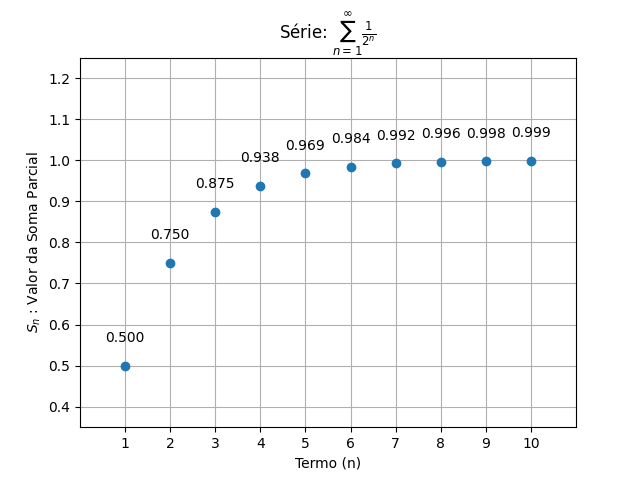
\includegraphics[width=0.7\textwidth]{../images/serie_1.png}
			\caption{Soma dos n primeiros termos da série  $  \displaystyle\sum_{n=1}^{\infty} \frac{1}{2^n}$}
		\end{figure}
	\end{frame}
	
	\section{Convergência e Divergência}
	\begin{frame}
		\tableofcontents[currentsection]
	\end{frame}
	
	\begin{frame}{Convergência e Divergência}
		\justifying
		\begin{itemize}
			\item \textbf{Convergência:} Uma série $\displaystyle\sum a_n$ converge se $\displaystyle\lim_{n \to \infty} s_n = s$.
			\item \textbf{Divergência:} Uma série diverge se não converge.
		\end{itemize}
	\end{frame}
	\begin{frame}{Convergência e Divergência}
		\begin{definition}[2]
			Dada uma série $\displaystyle\sum_{n=1}^{\infty} a_n = a_1 + a_2 + a_3 + \dots$, denote por $s_n$ sua $n$-ésima soma parcial:
			
			\centering {
				
				$s_n = \displaystyle\sum_{i=1}^{n} a_i = a_1 + a_2 + a_3 + \dots + a_n$}
			
			\justifying
			Se a sequência $\{s_n\}$ for convergente e $\displaystyle\lim_{n \to \infty}
			s_n = s$ existir como um número real, então a série $\displaystyle\sum a_n$ é
			chamada \textbf{convergente}, e escrevermos
			
			\centering {
				$a_1 + a_2 + a_3 + \dots + a_n + \dots = s$ ou $\displaystyle\sum_{n=1}^{\infty} a_n = s$
			}
			
			\justifying
			O número $s$ é chamado a \textbf{soma} da série. Se a sequência $\{s_n\}$ é
			divergente, então a série é chamada \textbf{divergente}.
		\end{definition}
	\end{frame}
	\begin{frame}{Convergência e Divergência}
		\begin{observation}[1]
			\justifying
			A soma de uma série é o limite da sequência de somas parciais. Desse modo, quando escrevermos $\displaystyle\sum_{n=1}^{\infty} a_n = s$, queremos dizer que, somando um número suficiente de termos da série, podemos chegar tão perto quanto quisermos do número $s$. Observe que
			
			$$\displaystyle\sum_{n=1}^{\infty} a_n = \lim_{n \to \infty}s_n = \lim_{n \to \infty} \sum_{i=1}^{n} a_i.$$
		\end{observation}
	\end{frame}
	\begin{frame}{Convergência e Divergência}
		
		Vamos analisar a série $\displaystyle\sum_{n=1}^{\infty} \frac{1}{2^n}$ que foi
		apresentada anteriormente, com o objetivo de determinar se essa série converge
		ou diverge. Para isso, vamos examinar algumas das somas parciais. A primeira
		soma parcial é $s_1 = \frac{1}{2}$, a segunda é $s_2 = \frac{1}{2} +
		\frac{1}{4} = \frac{3}{4}$, e a terceira é $s_3 = \frac{1}{2} + \frac{1}{4} +
		\frac{1}{8} = \frac{3}{4} + \frac{1}{8} = \frac{7}{8}$, e assim sucessivamente.
	\end{frame}
	\begin{frame}{Convergência e Divergência}
		
		Observe que $s_n$ pode ser escrito como $s_n = \frac{2^n - 1}{2^n} = 1 -
		\frac{1}{2^n}$. Como a soma de uma série é o limite da sequência de somas
		parciais, podemos então escrever $s_n$ como $\displaystyle\lim_{i \to \infty} 1
		- \frac{1}{2^i} = 1$. Como o limite existe e é um número real, então dizemos
		que a série $\displaystyle\sum_{n=1}^{\infty} \frac{1}{2^n}$ é convergente,
		convergindo para 1.
	\end{frame}
	\begin{frame}{Convergência e Divergência}
		\begin{figure}
			\centering
			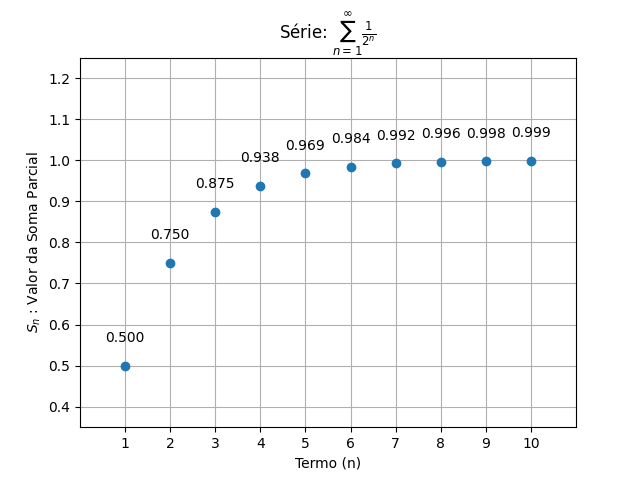
\includegraphics[width=0.7\textwidth]{../images/serie_1.png}
			\caption{Soma dos n primeiros termos da série  $  \displaystyle\sum_{n=1}^{\infty} \frac{1}{2^n}$}
		\end{figure}
	\end{frame}
	\begin{frame}{Convergência e Divergência}
		
		Vamos analisar a série $\displaystyle\sum_{n=1}^{\infty} log (\frac{n}{n +
			1})$, com o objetivo de determinar se essa série converge ou diverge. Seguindo
		o método anterior, vamos pegar algumas somas parciais desta série. A primeira
		soma parcial é $s_1 = log \frac{1}{2}$, a segunda é $s_2 = log \frac{1}{2} +
		log \frac{2}{3} = log \frac{1}{3}$, e a terceira é $s_3 = log \frac{1}{2} + log
		\frac{2}{3} + log \frac{3}{4} = log \frac{1}{3} + log \frac{3}{4} = log
		\frac{1}{4}$, e assim sucessivamente.
	\end{frame}
	\begin{frame}{Convergência e Divergência}
		
		Observe que $s_n$ pode ser escrito como $s_n = log \frac{1}{n + 1} = -log(n
		+1)$. Como a soma de uma série é o limite da sequência de somas parciais,
		podemos então escrever $s_n$ como $\displaystyle\lim_{i \to \infty} -log(n +1)
		= -\infty$. Como o limite não existe, dizemos que e série
		$\displaystyle\sum_{n=1}^{\infty} log (\frac{n}{n + 1})$ é divergente.
	\end{frame}
	\begin{frame}{Convergência e Divergência}
		\begin{figure}
			\centering
			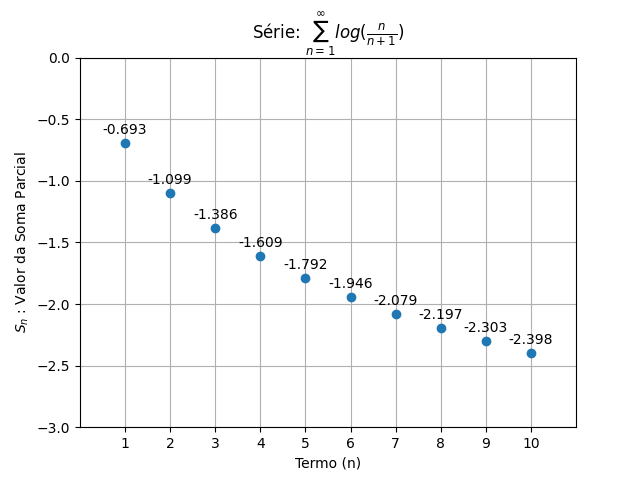
\includegraphics[width=0.7\textwidth]{../images/serie_2.png}
			\caption{Soma dos n primeiros termos da série  $  \displaystyle\sum_{n=1}^{\infty} log (\frac{n}{n + 1})$}
		\end{figure}
	\end{frame}
	
	\section{Propriedades das Séries Convergentes}
	\begin{frame}
		\tableofcontents[currentsection]
	\end{frame}
	
	\begin{frame}{Propriedades das Séries Convergentes}
		
		\begin{theorem}[1]
			Se a série $\displaystyle\sum_{n=1}^{\infty} a_n$ for convergente, então $\displaystyle\lim_{n \to \infty} a_n = 0$
		\end{theorem}
	\end{frame}
	\begin{frame}{Propriedades das Séries Convergentes}
		
		\justifying
		Seja $s_n = a_1 + a_2 + \dots + a_n$. Então, $a_n = s_n - s_{n - 1}$. Como $\displaystyle\sum_{n=1}^{\infty} a_n$ é convergente, a sequência $\{s_n\}$ é convergente. Seja $\displaystyle\lim_{n \to \infty} s_n = s$. Como $n - 1\rightarrow \infty$ quando $n \rightarrow \infty$, também temos $\displaystyle\lim_{n \to \infty} s_{n - 1} = s$. Portanto
		
		$\newline$
		
		\centering
		$\displaystyle\lim_{n \to \infty} a_n = \lim_{n \to \infty} (s_n - s_{n - 1})= \lim_{n \to \infty}  s_n - \lim_{n \to \infty}  s_{n - 1} = s - s = 0$
	\end{frame}
	
	\begin{frame}{Propriedades das Séries Convergentes}
		
		\begin{observation}[2]
			\justifying
			Com qualquer série $\displaystyle\sum_{n=1}^{\infty} a_n$ associamos duas sequências: a sequência $\{s_n\}$ de suas somas parciais e a sequência $\{a_n\}$ de seus termos. Se $\displaystyle\sum_{n=1}^{\infty} a_n$ for convergente, o limite da sequência $\{s_n\}$ é $s$ (a soma da série) e, como o Teorema (1) afirma, o limite da sequência $\{a_n\}$ é 0.
		\end{observation}
	\end{frame}
	
	\begin{frame}{Propriedades das Séries Convergentes}
		\justifying
		Considerando o Teorema (1), vamos analisar novamente a série $\displaystyle\sum_{n=1}^{\infty} \frac{1}{2^n}$. Podemos  verificar que $\displaystyle\lim_{n \to \infty} \frac{1}{2^n} = 0$, o que sugere a convergência da série. De fato, como já observamos, esta é uma série convergente.
	\end{frame}
	\begin{frame}{Propriedades das Séries Convergentes}
		\justifying
		Agora, consideremos a série $\displaystyle\sum_{n=1}^{\infty} \log \left(\frac{n}{n+1}\right)$. Primeiramente, analisamos o termo individual da série no infinito. Encontramos que $\displaystyle\lim_{n \to \infty} \log \left(\frac{n}{n+1}\right) = \log \left(\lim_{n \to \infty} \frac{n}{n+1}\right)$. Simplificando a expressão $\frac{n}{n+1}$, chegamos a $1 - \frac{1}{n+1}$, e no limite isso se aproxima de 1. Portanto, aplicando a propriedade do logaritmo que diz que o logaritmo de 1 é zero, temos:
		
		$$\lim_{n \to \infty} \log \left(\frac{n}{n+1}\right) = \lim_{n \to \infty} \log (1 - \frac{1}{n+1}) = \log (1) = 0$$
	\end{frame}
	\begin{frame}{Propriedades das Séries Convergentes}
		\justifying
		Assim como para o caso da série anterior, o fato de que o termo individual tende a zero é um indicativo necessário, mas não suficiente, para determinar a convergência da série. No entanto, diferente da série $\displaystyle\sum_{n=1}^{\infty} \frac{1}{2^n}$, que é uma série geométrica claramente convergente, a convergência ou divergência da série $\displaystyle\sum_{n=1}^{\infty} \log \left(\frac{n}{n+1}\right)$ não é imediatamente aparente apenas com esta informação, e requer uma análise mais detalhada.
		
	\end{frame}
	\begin{frame}{Propriedades das Séries Convergentes}
		
		\begin{observation}[3]
			\justifying
			Se $\displaystyle\lim_{n \to \infty} a_n = 0$, não podemos concluir que $\displaystyle\sum_{n=1}^{\infty}a_n$ é convergente.
			
			Se $\displaystyle\lim_{n \to \infty} a_n$ não existir ou se
			$\displaystyle\lim_{n \to \infty} a_n \neq 0$, então a série
			$\displaystyle\sum_{n=1}^{\infty}a_n$ é divergente.
		\end{observation}
		
		\small{Teste de Divergência}
	\end{frame}
	\begin{frame}{Propriedades das Séries Convergentes}
		\begin{theorem}[2]
			
			Seja $c$ uma constante e $\displaystyle\sum_{n=1}^{\infty} a_n$ uma série
			convergente. Então $\displaystyle\sum_{n=1}^{\infty} ca_n$ é também convergente
			e é igual a $c \displaystyle\sum_{n=1}^{\infty} a_n$
			
		\end{theorem}
	\end{frame}
	\begin{frame}{Propriedades das Séries Convergentes}
		
		Seja $\displaystyle\sum_{n=1}^{\infty} a_n$, uma série convergente, então por
		definição:
		
		$$s = \lim_{n \to \infty}s_n = \lim_{n \to \infty} \sum_{i=1}^{n} a_i.$$
		
		Então, considerando $c$ uma constante, temos que:
		
		$$\lim_{n \to \infty} \sum_{i=1}^{n} ca_i = \lim_{n \to \infty} c \sum_{i=1}^{n} a_i = c \lim_{n \to \infty} \sum_{i=1}^{n} a_i= cs.$$
		
		Portanto, $\displaystyle\sum_{n=1}^{\infty} ca_n$ é convergente e é igual a $c
		\displaystyle\sum_{n=1}^{\infty} a_n$.
		
	\end{frame}
	\begin{frame}{Propriedades das Séries Convergentes}
		\begin{theorem}[3]
			
			Se $\displaystyle\sum_{n=1}^{\infty} a_n$ e $\displaystyle\sum_{n=1}^{\infty}
			b_n$ são séries convergentes, então $\displaystyle\sum_{n=1}^{\infty} (a_n +
			b_n)$ é também convergente e é igual a $\displaystyle\sum_{n=1}^{\infty} a_n +
			\sum_{n=1}^{\infty} b_n$.
			
		\end{theorem}
	\end{frame}
	\begin{frame}{Propriedades das Séries Convergentes}
		
		Sejam $A = \displaystyle\sum_{n=1}^{\infty} a_n$ e $B =
		\displaystyle\sum_{i=n}^{\infty} b_n$, então por definição:
		
		$$A = \lim_{n \to \infty} \sum_{i=1}^{n} a_i \text{ e } B = \lim_{n \to \infty} \sum_{i=1}^{n} b_i.$$
		
		Considere a soma de $A$ e $B$:
		
		$$A + B = \lim_{n \to \infty} \sum_{i=1}^{n} a_i + \lim_{n \to \infty} \sum_{i=1}^{n} b_i = \lim_{n \to \infty} \left( \sum_{i=1}^{n} a_i + \sum_{i=1}^{n} b_i \right)$$$$ = \lim_{n \to \infty} \sum_{i=1}^{n} (a_i + b_i).$$
		
		Logo, $\displaystyle\sum_{n=1}^{\infty} (a_n + b_n)$ é convergente e igual a
		$\displaystyle\sum_{n=1}^{\infty} a_n + \displaystyle\sum_{n=1}^{\infty} b_n$.
		
	\end{frame}
	
	\begin{frame}{Propriedades das Séries Convergentes}
		\begin{theorem}[4]
			
			Se $\displaystyle\sum_{n=1}^{\infty} a_n$ e $\displaystyle\sum_{n=1}^{\infty}
			b_n$ são séries convergentes, então $\displaystyle\sum_{n=1}^{\infty} (a_n -
			b_n)$ é também convergente e é igual a $\displaystyle\sum_{n=1}^{\infty} a_n -
			\displaystyle\sum_{n=1}^{\infty} b_n$.
			
		\end{theorem}
	\end{frame}
	\begin{frame}{Propriedades das Séries Convergentes}
		Utilizando a mesma lógica do Teorema (3), temos:
		
		$$A - B = \lim_{n \to \infty} \sum_{i=1}^{n} a_i - \lim_{n \to \infty} \sum_{i=1}^{n} b_i = \lim_{n \to \infty} \left( \sum_{i=1}^{n} a_i - \sum_{i=1}^{n} b_i \right) $$$$= \lim_{n \to \infty} \sum_{i=1}^{n} (a_i - b_i).$$
		
		Assim, $\displaystyle\sum_{n=1}^{\infty} (a_n - b_n)$ é convergente e igual a
		$\displaystyle\sum_{n=1}^{\infty} a_n - \displaystyle\sum_{n=1}^{\infty} b_n$.
	\end{frame}
	\begin{frame}{Propriedades das Séries Convergentes}
		
		\begin{example}[1]
			Calcule a soma da série $\displaystyle\sum_{n=1}^{\infty} \left(\frac{3}{n(n + 1)} + \frac{1}{2^n}\right)$.
		\end{example}
		
	\end{frame}
	
	\begin{frame}{Propriedades das Séries Convergentes}
		\justifying
		Pelo Teorema (3), podemos escrever
		$$\displaystyle\sum_{n=1}^{\infty} \left(\frac{3}{n(n + 1)} + \frac{1}{2^n}\right) = \displaystyle\sum_{n=1}^{\infty} \frac{3}{n(n + 1)} + \displaystyle\sum_{n=1}^{\infty} \frac{1}{2^n}$$.
		
		Pelo Teorema (2), podemos escrever $$ \displaystyle\sum_{n=1}^{\infty}
		\frac{3}{n(n + 1)} + \displaystyle\sum_{n=1}^{\infty} \frac{1}{2^n} =
		3\displaystyle\sum_{n=1}^{\infty} \frac{1}{n(n + 1)} +
		\displaystyle\sum_{n=1}^{\infty} \frac{1}{2^n}$$.
	\end{frame}
	
	\begin{frame}{Propriedades das Séries Convergentes}
		Note que podemos escrever,
		$$\displaystyle\sum_{n=1}^{\infty} \frac{1}{n(n + 1)} = \displaystyle\sum_{n=1}^{\infty} \left(\frac{1}{n} - \frac{1}{n + 1}\right)$$
		no qual seu $s_n$ será:
		$$\displaystyle\sum_{i=1}^{n} \left(\frac{1}{i} - \frac{1}{i + 1}\right) = \left(1 - \frac{1}{2}\right) + \left(\frac{1}{2} - \frac{1}{3}\right) + \left(\frac{1}{3} - \frac{1}{4}\right) + \dots + \left(\frac{1}{n} - \frac{1}{n + 1}\right)$$
		$ = 1 - \displaystyle\frac{1}{n + 1} $, logo $\displaystyle\lim_{n \to \infty} \left(1 - \frac{1}{n + 1}\right) = 1$
	\end{frame}
	
	\begin{frame}{Propriedades das Séries Convergentes}
		Assim, obtemos que $\displaystyle\sum_{n=1}^{\infty} \frac{1}{n(n + 1)} = 1$, e já verificamos anteriormente que $\displaystyle\sum_{n=1}^{\infty} \frac{1}{2^n} = 1$, desta forma, podemos escrever
		$$\displaystyle\sum_{n=1}^{\infty} \left(\frac{3}{n(n + 1)} + \frac{1}{2^n}\right) = 3\displaystyle\sum_{n=1}^{\infty} \frac{1}{n(n + 1)} + \displaystyle\sum_{n=1}^{\infty} \frac{1}{2^n} = 3\cdot1 + 1 = 4$$
	\end{frame}
	
	\begin{frame}{Propriedades das Séries Convergentes}
		\begin{figure}
			\centering
			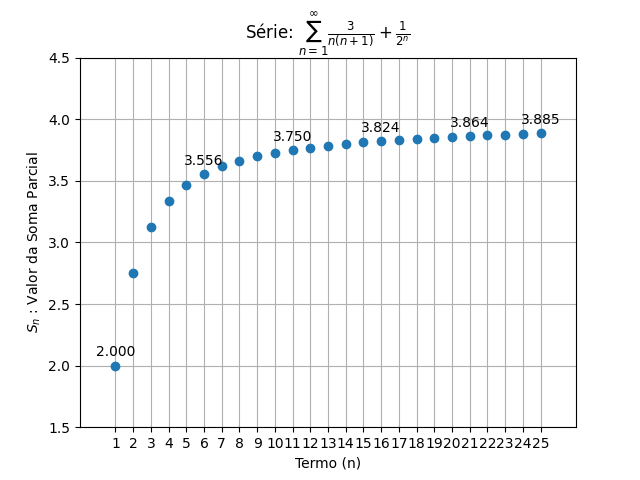
\includegraphics[width=0.7\textwidth]{../images/serie_3.png}
			\caption{Soma dos n primeiros termos da série  $\displaystyle\sum_{n=1}^{\infty} \left(\frac{3}{n(n + 1)} + \frac{1}{2^n}\right)$}
		\end{figure}
	\end{frame}
	
	\section{Séries Alternadas}
	\begin{frame}
		\tableofcontents[currentsection]
	\end{frame}
	
	\begin{frame}{Séries Alternadas}
		\begin{definition}[3]
			Uma \textbf{série alternada} é aquela cujos termos são alternadamente positivos e negativos. Aqui
			estão dois exemplos:
			
			$$
			1 - \frac{1}{2} + \frac{1}{3} - \frac{1}{4} + \frac{1}{5} - \frac{1}{6} + \dots = \displaystyle\sum_{n=1}^{\infty}(-1)^{n - 1}\frac{1}{n}
			$$
			
			$$
			- \frac{1}{2} +  \frac{2}{3} - \frac{3}{4} + \frac{4}{5} - \frac{5}{6} + \frac{6}{7} + \dots = \displaystyle\sum_{n=1}^{\infty}(-1)^{n}\frac{n}{n + 1}
			$$
			
			Vemos desses exemplos que o $n$-ésimo termo de uma série alternada é da forma
			
			$$a_n = (-1)^{n - 1}b_n \text{ ou } a_n = (-1)^{n}b_n$$
			
			onde $b_n$ é um número positivo. (De fato, $b_n = |a_n|$)
			
		\end{definition}
		
		% Apresente e demonstre brevemente o Teorema do Teste de Leibniz.
	\end{frame}
	
	\begin{frame}{Séries Alternadas}
		
		\begin{theorem}[4]
			\justifying
			Se a série alternada
			
			$$\displaystyle\sum_{n=1}^{\infty}(-1)^{n - 1} b_n = b_1 - b_2 + b_3 - b_4 + b_5 - b_6 + \cdots  $$
			
			Com $b_n > 0$ satisfaz
			
			\begin{itemize}[label=, left=115pt]
				\item (i) $b_{n + 1} \leq b_n$ para todo $n$
				\item (ii) $\displaystyle\lim_{n \to \infty} b_n = 0$
			\end{itemize}
			então a série é convergente.
			
		\end{theorem}
		\small{
			Este é o critério de convergência para séries alternadas, comumente conhecido como o Teste de Leibniz.}
		
	\end{frame}
	
	\begin{frame}{Séries Alternadas}
		Para as somas parciais pares, temos que:
		\begin{align*}
			& s_{2} = b_1 - b_2 \geq 0                                                                                    \\
			& s_{4} = (b_1 - b_2) + (b_3 - b_4) \geq s_2                                                                  \\
			& \quad \vdots                                                                                                \\
			& s_{2n} = (b_1 - b_2) + (b_3 - b_4) + \cdots + (b_{2n-1} - b_{2n})                                           \\
			& \text{\hspace{0.5cm}}= s_{2n-2} + (b_{2n-1} - b_{2n})                                                       \\
			& \text{\hspace{0.5cm}}= b_1 - (b_2 - b_3) - (b_4 - b_5) - \cdots - (b_{2n-2} - b_{2n-1}) - b_n \geq s_{2n-2}
		\end{align*}
		A sequência das somas parciais pares é crescente e limitada superiormente, uma vez que para cada termo subtraído, existe um termo não maior que este adicionado antes.
	\end{frame}
	
	\begin{frame}{Séries Alternadas}
		Para as somas parciais ímpares, observamos que:
		\begin{align*}
			& s_{1} = b_1                                                  \\
			& s_{3} = s_{2} + b_3 \leq s_{2} + b_2 = s_{1}                 \\
			& s_{5} = s_{4} + b_5 \leq s_{4} + b_4 = s_{3}                 \\
			& \quad \vdots                                                 \\
			& s_{2n+1} = s_{2n} + b_{2n+1} \leq s_{2n} + b_{2n} = s_{2n-1}
		\end{align*}
		A sequência das somas parciais ímpares é decrescente e limitada inferiormente por zero.
		
	\end{frame}
	
	\begin{frame}{Séries Alternadas}
		Dado que $b_n \to 0$, a diferença entre uma soma parcial ímpar e a soma parcial par anterior tende a zero, e assim as sequências de somas parciais pares e ímpares convergem para o mesmo limite. Isso mostra que a série alternada é convergente
	\end{frame}
	
	\begin{frame}{Séries Alternadas}
		\begin{figure}
			\centering
			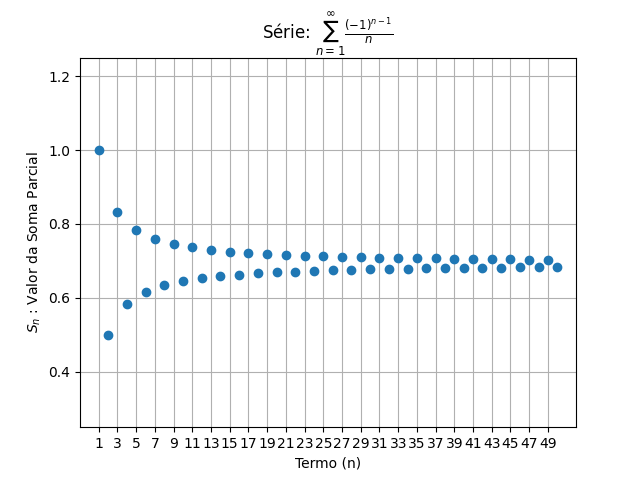
\includegraphics[width=0.7\textwidth]{../images/serie_4.png}
			\caption{Soma dos n primeiros termos da série  $\displaystyle\sum_{n=1}^{\infty} \frac{(-1)^{n-1}}{n}$}
		\end{figure}
	\end{frame}
	
	\begin{frame}{Séries Alternadas}
		Observe que $$\displaystyle\sum_{n=1}^{\infty} \frac{(-1)^{n-1}}{n} = 1 - \frac{1}{2} + \frac{1}{3} - \frac{1}{4} + \dots$$
		satisfaz a condição $(i)$ do Teorema (4), $b_{n + 1} \leq b_n$ para todo $n$, também, satisfaz a condição $(ii)$: $\displaystyle\lim_{n \to \infty} \frac{1}{n} = 0$. Logo, a série harmônica alternada é convergente.
	\end{frame}
	
	\section{Conclusão}
	\begin{frame}
		\tableofcontents[currentsection]
	\end{frame}
	
	\begin{frame}{Conclusão}
		
		\justifying
		Nesta apresentação, exploramos as séries numéricas, um conceito fundamental no estudo da matemática avançada, especialmente em análise e cálculo. Discutimos o que são séries numéricas, como identificar a convergência e a divergência de uma série e também examinamos propriedades importantes das séries convergentes. Por meio do Teorema do Teste de Leibniz, analisamos as séries alternadas, uma categoria especial de séries que seguem um padrão de sinais alternados.
		
	\end{frame}
	
	\begin{frame}{Conclusão}
		\justifying
		
		A compreensão das séries numéricas nos permite resolver diversos problemas
		matemáticos e aplicar esses conceitos em situações práticas, incluindo a
		modelagem matemática em física, economia e outras ciências aplicadas. A
		habilidade de discernir entre séries convergentes e divergentes é uma
		ferramenta valiosa para garantir a validade e a aplicabilidade dos resultados
		obtidos.
		
	\end{frame}
	\begin{frame}{Conclusão}
		
		\justifying
		
		Esperamos que esta apresentação tenha esclarecido alguns dos aspectos
		importantes das séries numéricas e que você esteja agora mais confortável com o
		tema. A matemática das séries numéricas é vasta e repleta de nuances e
		esperamos ter despertado o seu interesse para aprofundar-se mais nestes
		estudos. Obrigado por sua participação e atenção durante a apresentação.
	\end{frame}
	\begin{frame}{Perguntas?}
		\centering
		\Large
		Obrigado pela atenção!\\
		Perguntas?
	\end{frame}
	
\end{document}

